\begin{figure}[htbp]
    \centering

    \begin{subfigure}{0.48\textwidth}
        \centering
        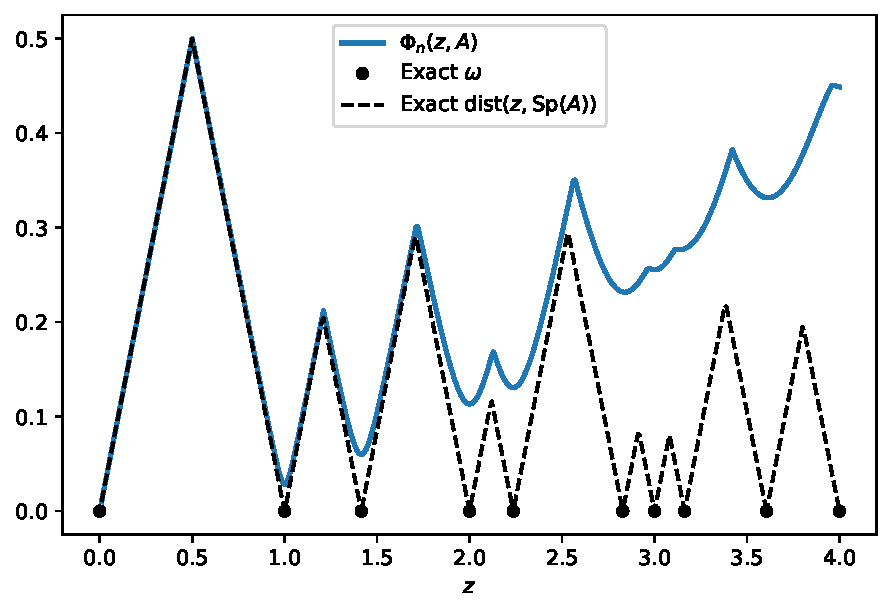
\includegraphics[width=\textwidth]{images/dist_plot_N=32.pdf}
        \caption{$N=32$}
        \label{fig:maxwell-dist-N32}
    \end{subfigure}
    \hfill
    % \begin{subfigure}{0.32\textwidth}
    %     \centering
    %     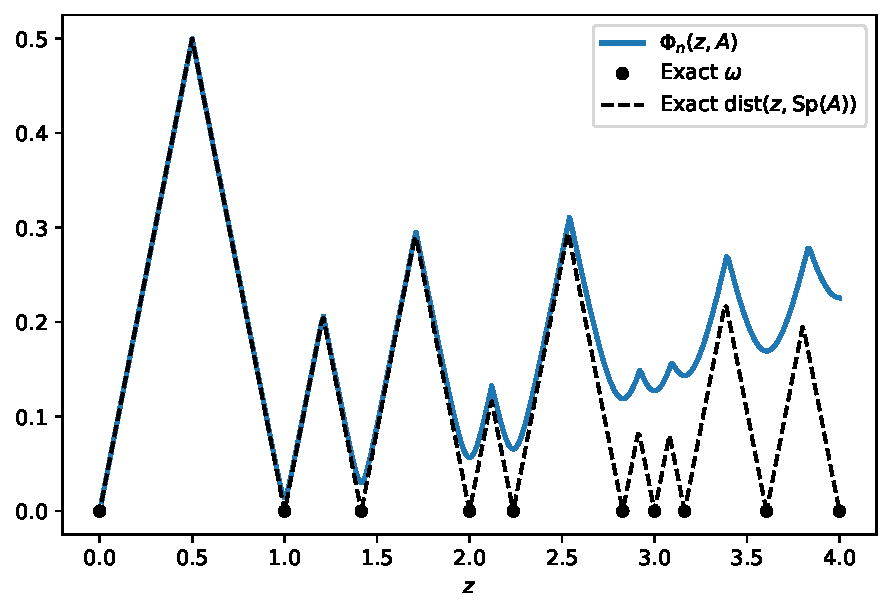
\includegraphics[width=\textwidth]{images/dist_plot_N=64.pdf}
    %     \caption{$N=64$}
    %     \label{fig:maxwell-dist-N64}
    % \end{subfigure}
    % \hfill
    \begin{subfigure}{0.48\textwidth}
        \centering
        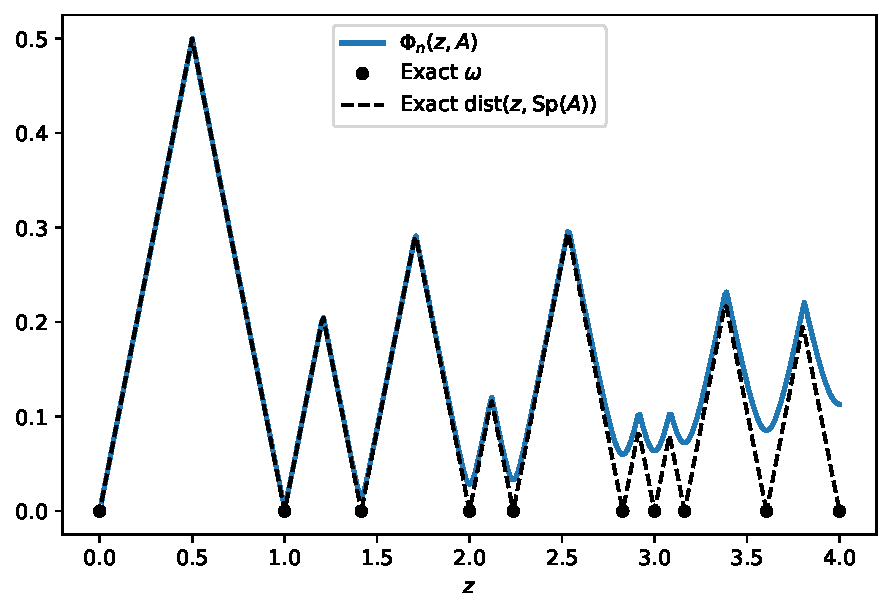
\includegraphics[width=\textwidth]{images/dist_plot_N=128.pdf}
        \caption{$N=128$}
        \label{fig:maxwell-dist-N128}
    \end{subfigure}

    \caption{Results from applying Colbrook's algorithm to the Maxwell operator \eqref{max op}.}
    \label{FirstMatt}
\end{figure}